\begin{example}[Advection 2D]
    \label{ex:adv2D_kriv}
    In $\Omega = \langle -1, 1 \rangle^2$ we will solve equation \eqref{eq:ex_advection}.
    We choose the same initial conditions $u(0, x)$ as in \cite{Krivodonova2007}
    \begin{equation}
        u(x, 0) =\begin{cases}
        cos^2(2\pi r), \quad r \leq 0.25,\\
        1, \quad 0.1 \leq x \leq 0.6 and -0.25 \leq y \leq 0.25,\\
        0, \quad \mathrm{elsewhere},
        \end{cases}
    \end{equation}
    where $r = (x + 0.5)^2 + y$. We choose the velocity $\vec{a}$ dependent on space 
    coordinates:
    $$
    \vec{a} = (2\pi x, -2\pi y),
    $$
    so that the initial data rotate about the origin. Revolving fully for every integer 
    value of $t$. In \Cref{fig:sol_3D_adv2D} we can see comparison of initial state and 
    state after one revolution. In \Cref{tab:errs_adv2D} and \Cref{fig:sol_cont_adv2D} we 
    present errors and contours of the solution for different orders, we choose mesh so 
    that the number of DOFs remains the same ($57600$) for each order. 
    \Cref{tab:errs_adv2D} clearly shows that higher orders are not beneficial. And the 
    trade off between refining a mesh and increasing the order seems to favor mesh 
    refining.    
    \begin{table}[p!]
        \centering    
        \caption{\Cref{ex:adv2D_kriv}. Errors in $L^2$ norm for different orders.}    
        \label{tab:errs_adv2D}
        \begin{tabular}{lcccc}
            \toprule
            Order & \#Cells & $N_{base}$ & Error & Initial error \\ 
            \midrule
            1&$14400$&$ 4$&$0.1577$&$0.0004$\\
            2&$6400 $&$ 9$&$0.1963$&$0.0001$\\
            3&$3600 $&$16$&$0.2297$&$0.0648$\\
            4&$2304 $&$25$&$0.2619$&$0.0787$\\
            \bottomrule 
        \end{tabular} 
    \end{table}
\end{example}

\begin{figure}[h!]
    \centering
    \begin{subfigure}{.5\textwidth}	
        \centering	
        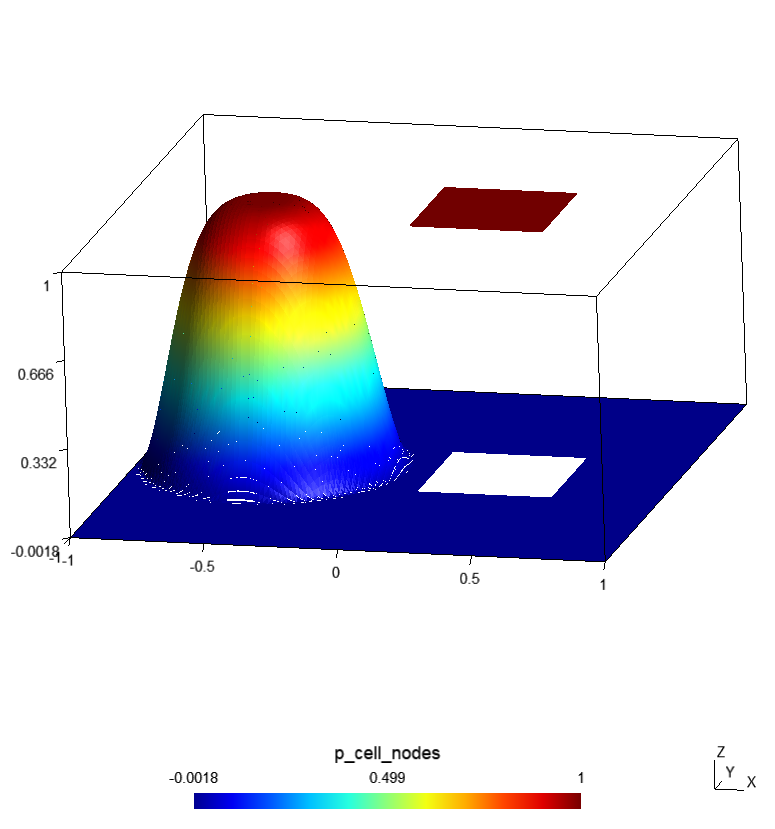
\includegraphics[width=\linewidth]{../figs/sols/kriv-sol0-3d-h14400o01}
        \caption{$t = 0$}
    \end{subfigure}%
    \begin{subfigure}{.5\textwidth}
        \centering	
        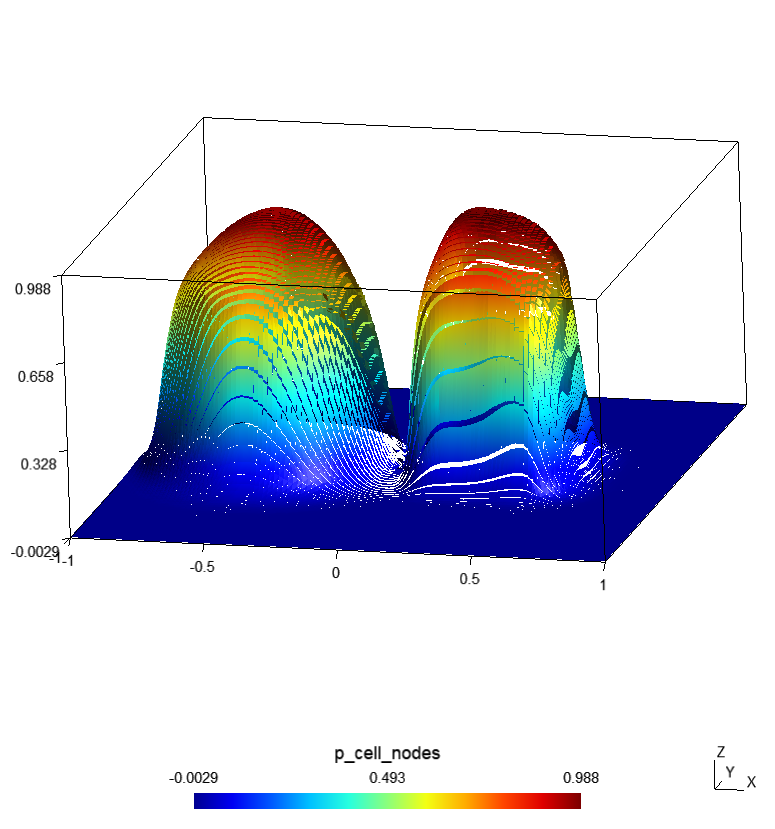
\includegraphics[width=\linewidth]{../figs/sols/kriv-sol-3d-h14400o01}
        \caption{$t = 1$}
    \end{subfigure}
    \caption{\Cref{ex:adv2D_kriv}.  Approximation of initial condition (left) and 
    solution after one revolution (right) obtained using first order approximation.}
    \label{fig:sol_3D_adv2D}
\end{figure}

\begin{figure}[p!]
    \centering
    \begin{subfigure}{.5\textwidth}	
        \centering	
        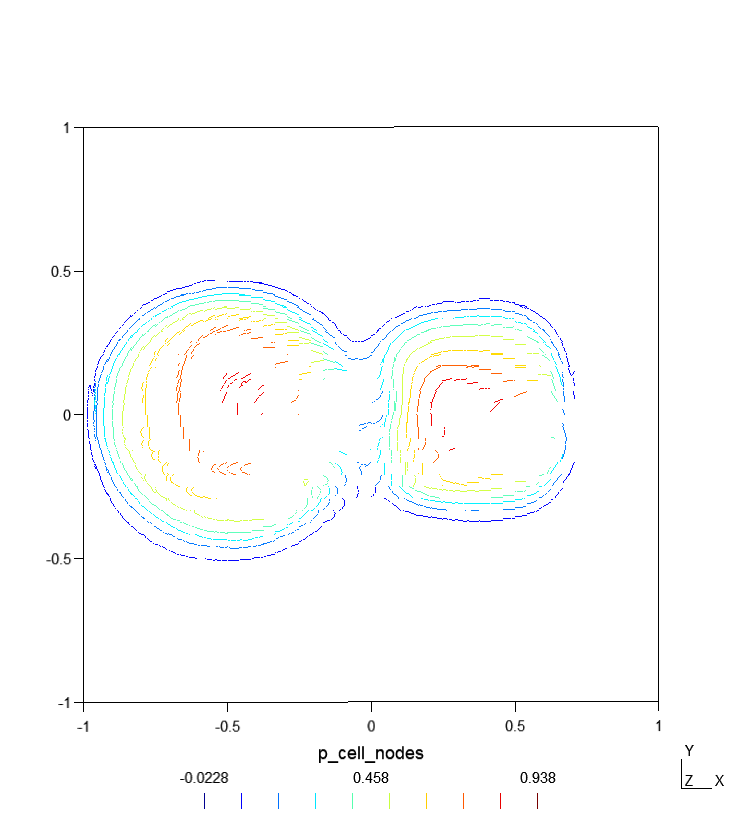
\includegraphics[width=\linewidth]{../figs/sols/kriv-sol-h2304o04}
        \caption{$M=4$}
    \end{subfigure}%
    \begin{subfigure}{.5\textwidth}
        \centering	
        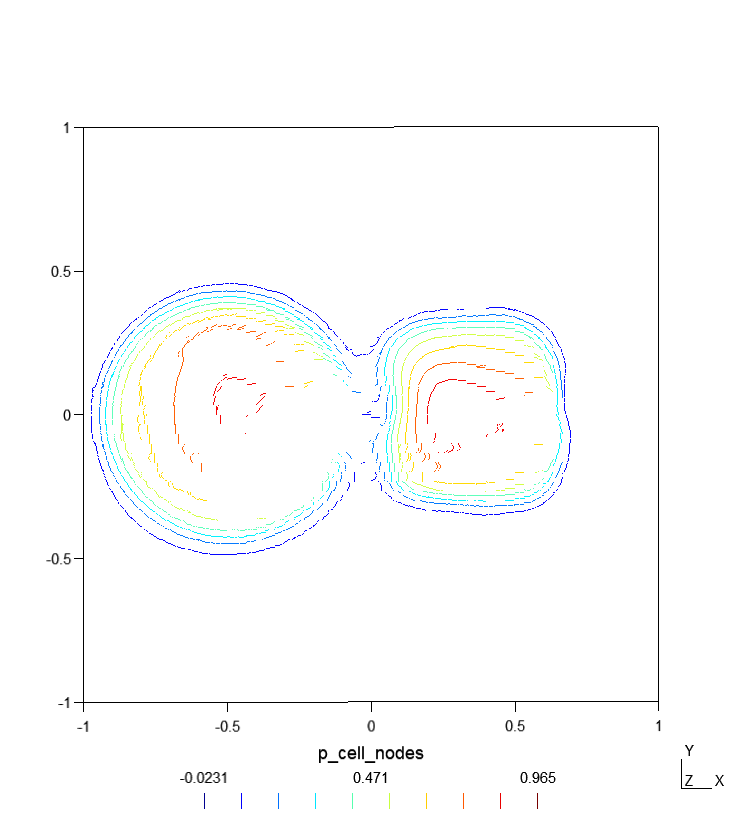
\includegraphics[width=\linewidth]{../figs/sols/kriv-sol-h3600o03}
        \caption{$M = 3$}
    \end{subfigure}
    \begin{subfigure}{.5\textwidth}	
        \centering	
        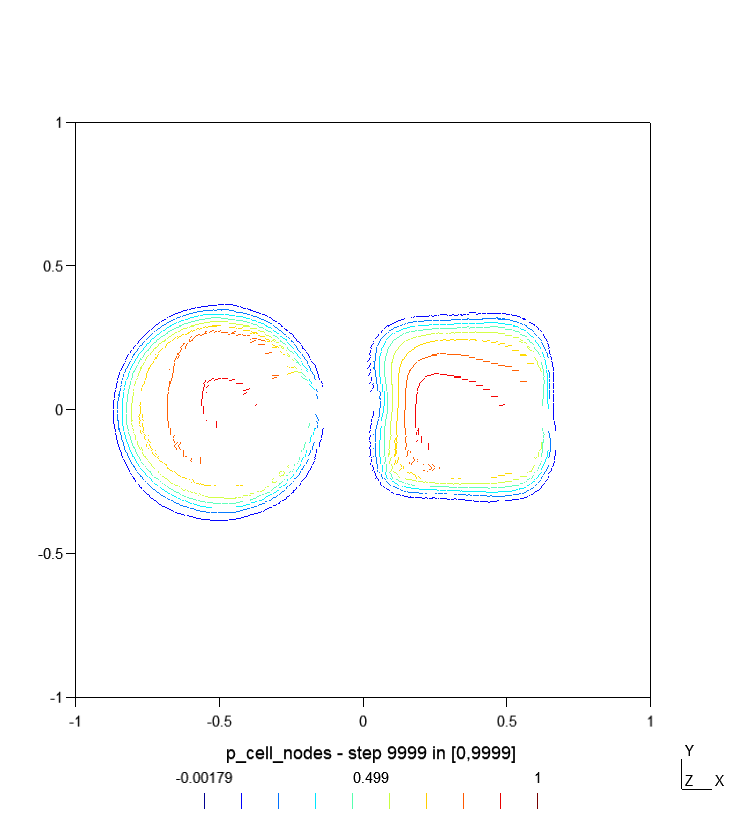
\includegraphics[width=\linewidth]{../figs/sols/kriv-sol-h6400o02}
        \caption{$M=2$}
    \end{subfigure}%
    \begin{subfigure}{.5\textwidth}
        \centering	
        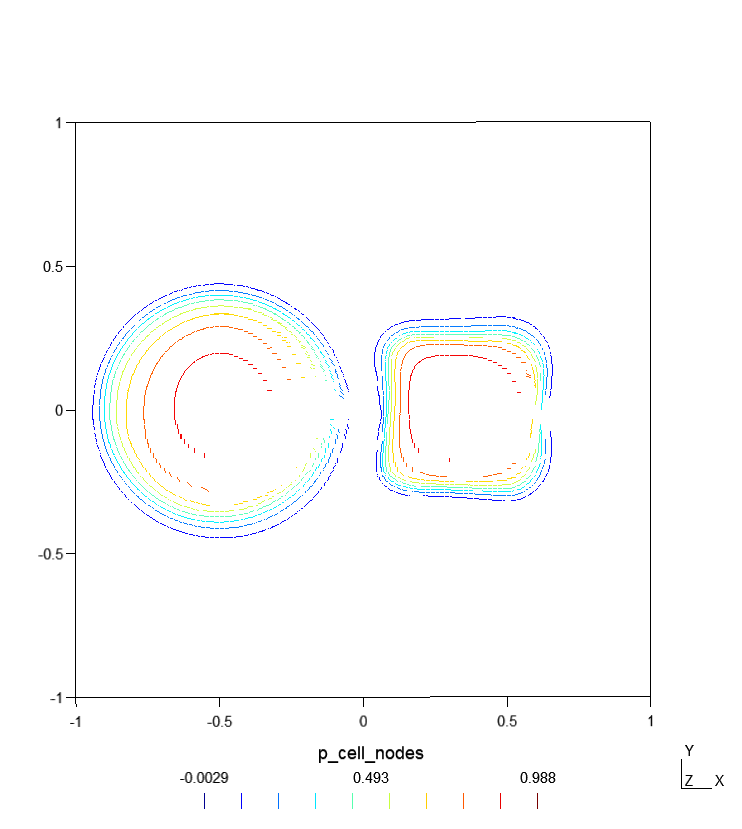
\includegraphics[width=\linewidth]{../figs/sols/kriv-sol-h14400o01}
        \caption{$M = 1$}
    \end{subfigure}
    \caption{\Cref{ex:adv2D_kriv}. Contours of the solution for different orders, number 
    of DOFs is kept constant.}
    \label{fig:sol_cont_adv2D}
\end{figure}


